\chapter{Modelo de iluminación\label{ch:iluminacion}}
En este capítulo vamos a ver los principios de los modelos de iluminación y algunos operadores importantes. Vamos a presentar el modelo de iluminación Phong, que sigue presente desde su publicación \cite{phong1975illumination}.
\begin{quote}{Bui Thoung Phong \cite{cite} (p. 1)}
    \enquote{La percepción visual humana y las leyes de la óptica, se consideran indispensables en el desarrollo de una regla de sombreado, proporcionando una mejor calidad y un mayor realismo en las imágenes generadas}.
\end{quote}
Dividiremos el capítulo en dos secciones, luces y sombras. Veremos que ambos hacen uso de la normal de la superficie, por ello, vamos a definir en \textit{GLSL}, la función de cálculo numérico visto en los \textit{Preliminares}\ref{sec:normal}.
\begin{lstlisting}
// Normal de la isosuperficie en p.
vec3 Normal(vec3 p){
     // f(x1,...,xn)
     float fxyz = escena_sdf(p);
     // f(x1,..,xi+h,xn)
     float fxhyz = escena_sdf(p + vec3(EPSILON, 0., 0.));
     float fxyhz = escena_sdf(p + vec3(0., EPSILON, 0.));
     float fxyzh = escena_sdf(p + vec3(0., 0., EPSILON));
     // Usamos la definicion de derivadas parciales para calcular el gradiente, proporcional a la normal en el punto
     return normalize(vec3(
         (fxhyz - fxyz) / EPSILON,
         (fxyhz - fxyz) / EPSILON,
         (fxyzh - fxyz) / EPSILON
     ));
}
\end{lstlisting}
\newpage
Vamos a ahora a presentar el operador, \textit{producto escalar},
definido en \textit{GLSL} como "\textit{dot}", formalmente, \(\cdot :\mathbb{R}^2\times\mathbb{R}^2\longrightarrow \mathbb{R}\) 
\[\Vec{v} \cdot  \Vec{r} = v_xr_x + v_yr_y + v_zr_z = \vert \vert\Vec{v}\vert\vert\vert \Vec{r}\vert\vert\cos(\Theta)\]
Si ambos son vectores están normalizados, \(\Vec{v} \cdot \Vec{r} = \cos(\alpha)\). El ángulo \(\Theta\), es el menor de los ángulos entre los dos vectores sobre el plano que forman en el origen. La imagen de este operador es \([-1,1]\), es fácil observar que, en vectores perpendiculares, el producto será cero y en caso de ser paralelos, este será \(\pm 1\) y el signo dependerá de la dirección de ambos. Con esta definición, podemos ahora presentar el operador de proyección de un vector \Vec{v} sobre otro \(\Vec{r}\), nos será muy útil de aquí en adelante:

\[\Vec{v} \cdot  \Vec{r} = \vert\vert \Vec{v}\vert\vert\vert \Vec{r}\vert\vert\cos(\Theta)\Longleftrightarrow \dfrac{\Vec{r} \cdot  \Vec{v}}{\vert\vert \Vec{r}\vert\vert} = \vert\vert v\vert\vert\cos(\Theta)\]
Utilizando la relación entre el cateto y la hipotenusa:
\[\cos(\Theta)=\dfrac{\vert\vert \text{proy}_{\Vec{r}}\Vec{v}\vert\vert}{\vert\vert \Vec{v}\vert\vert}\Longleftrightarrow \vert\vert \text{proy}_{\Vec{r}}\Vec{v}\vert\vert=\vert\vert \Vec{v}\vert\vert\cos(\Theta)=\dfrac{\Vec{r} \cdot  \Vec{v}}{\vert\vert \Vec{r}\vert\vert}\]
Finalmente, multiplicamos por el vector normalizado \(\text{norm}(r)\):
\[ \text{proy}_{\Vec{r}}\Vec{v}=\left(\dfrac{\Vec{v}\cdot\Vec{r}}{\vert\vert \Vec{r}\vert\vert}\right)\dfrac{\Vec{r}}{\vert\vert\Vec{r}\vert\vert}=\left(\dfrac{\Vec{v}\cdot\Vec{r}}{\vert\vert \Vec{r}\vert\vert^2}\right)\Vec{r}=\left(\dfrac{\Vec{v}\cdot \Vec{r}}{\Vec{r}\cdot \Vec{r}}\right)\Vec{r}\]

\begin{figure}[H]
  \centering
  \captionsetup{justification=centering}%,margin=2cm
  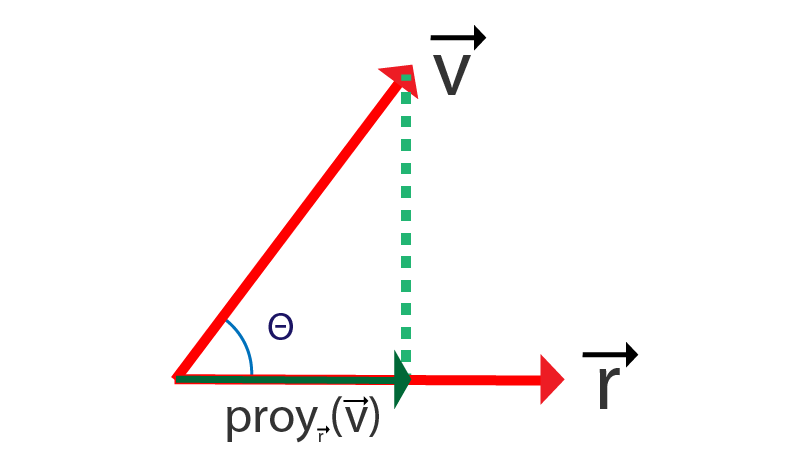
\includegraphics[width=0.5\textwidth]{secciones/imagenes/sdf/proofs/proyection.png}
  \caption{Proyección \(\Vec{v}\) sobre \(\Vec{r}\)}
  \label{fig:proyection}
\end{figure}
Una vez visto estos dos operadores, podemos presentar un nuevo operador, implementado de manera nativa en el lenguaje \textit{GLSL} y que es esenciales las definición de un modelo de iluminación:
\begin{table}[H]
    \begin{tabularx}{\textwidth}{l|X}
        \toprule
        Función & Definición\\
        \midrule
        \pbox{10cm}{
          reflect(\\
          \tab[1cm]vecN v,\\
          \tab[1cm]vecN n, \\
          )}& Operador de reflexión de un vector \(\Vec{v}\) sobre el vector normal \(\Vec{n}\), definido como:
        \[\Vec{r}=\Vec{v} - 2(\Vec{n} \cdot \Vec{v})\Vec{n}\]
        
        \begin{minipage}{1.0\textwidth}
          \centering
          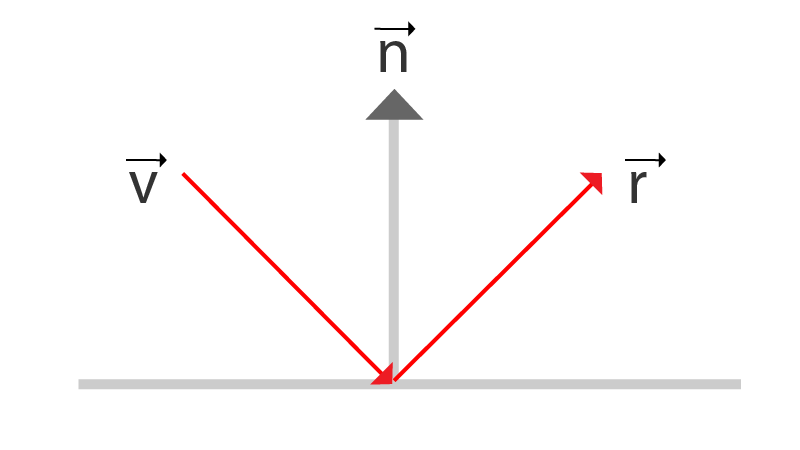
\includegraphics[width=.25\textwidth]{secciones/imagenes/lightmodel/reflect.png}
        \end{minipage}
        \\
        \bottomrule
    \end{tabularx}
    \caption{Operador de reflexión en GLSL \label{eq:reflexion}}
\end{table}

El operador de reflexión trabaja con tres vectores,  \(\Vec{n}\) un vector normal de la superficie, \(\Vec{v}\) el vector incidente y \(\Vec{r}\) el vector resultante. Observamos que, 
\(\vert\vert \Vec{r}-(-\Vec{v})\vert\vert = 2\vert\vert\text{proy}_{\Vec{n}}(\Vec{-v})\vert\vert\), por lo que calcularemos el vector a la normal, \(\Vec{d}=\text{proy}_{\Vec{n}}(\Vec{v}) - (-\Vec{v})\), finalmente, desplazaremos el vector \(\Vec{v}\) dos veces \(\Vec{d}\), como vimos en la equivalencia anterior.
\[\Vec{r}=(-\Vec{v}) + 2\Vec{d}=(-\Vec{v}) + 2(\text{proy}_{\Vec{n}}(-\Vec{v}) - (-\Vec{v}))= -2\text{proy}_{\Vec{n}}(\Vec{v}) + \Vec{v}\]
\section{Luz e Intensidad}
 Definimos la \textit{intensidad lumínica} en un punto como un factor multiplicativo al material asignado al punto de la \textit{isosuperficie}, representa cómo de iluminado está. Como es un factor multiplicativo, el valor de \(0.0\), representa la intensidad nula u oscuridad. Mientras que el valor \(1.0\) representa el valor más iluminado.\\\\ 
El operador \textit{producto escalar} nos debería dar una breve intuición del papel importante que juega en el cálculo de la intensidad. Como esta no puede ser negativa, definimos el operador producto escalar positivo y normalizado "\(\cdot_{[0,1]}\)".
\[\cdot_{[0,1]}:\mathbb{R}^2\times\mathbb{R}^2\longrightarrow[0,1], \Vec{a}\cdot_{[0,1]}\Vec{b}=\max\left(\dfrac{\Vec{a}\cdot \Vec{b}}{\vert\vert\Vec{a}\vert\vert\vert\vert \Vec{b}\vert\vert}, 0\right)\]
Vamos a presentar dos tipos de luces, \textit{radiales} y \textit{direccionales}, aplicados sobre  el "\textit{Modelo de Iluminación de Phong}", presentado en 1973 por \textit{Tuong Phong} como un modelo de iluminación empírico. Para ello, vamos a ver como el modelo se descompone en tres. 
\subsection{Intensidad ambiente}
Se trata de un valor \(I_a \in [0,1]\) que indica cuanto de iluminada está la isosuperficie, de manera inicial o si no hubieran luces. 
\begin{figure}[H]
  \centering
  \captionsetup{justification=centering}%,margin=2cm
   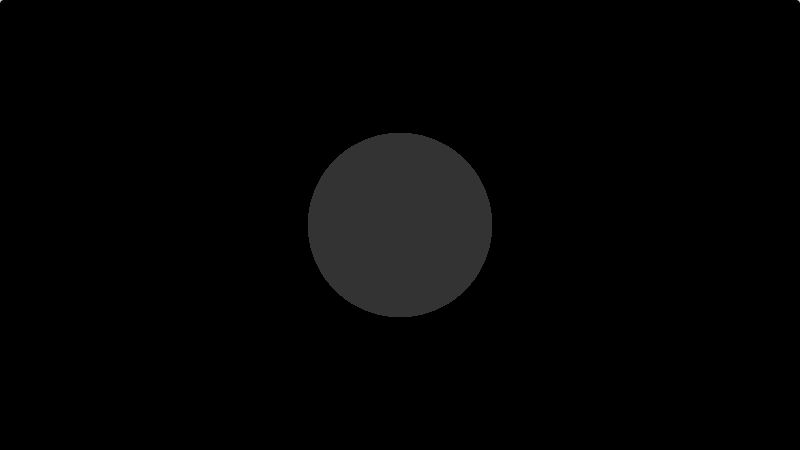
\includegraphics[width=1.0\textwidth]{secciones/imagenes/lightmodel/ambiental.png}
  \caption{Intensidad Ambiental sobre la esfera.}
  \label{fig:ambient}
\end{figure}

\subsection{Intensidad difusa}
Esta intensidad representa cuanta luz es refractada por la superficie en un punto \(\Vec{p}\) por cada una de las luces de la escena \(\Vec{l_i}\in L\), donde \(\Vec{l_i}\) representa la posición de la luz, se comprueba como incide la luz sobre la superficie, utilizando la normal \(\Vec{n}\) en el punto \(\Vec{p}\). 
\[I_d = \sum_{\Vec{l_i}\in L} \Vec{n}\cdot_{[0, 1]}(\Vec{l_i}-\Vec{p})\]
Es fácil observar que, la intensidad debería ser máxima cuando los rayos inciden en de manera paralela en sentido contrario al vector normal y nulo en caso de que sean perpendiculares u opuestos.
\begin{figure}[H]
  \centering
  \captionsetup{justification=centering}%,margin=2cm
  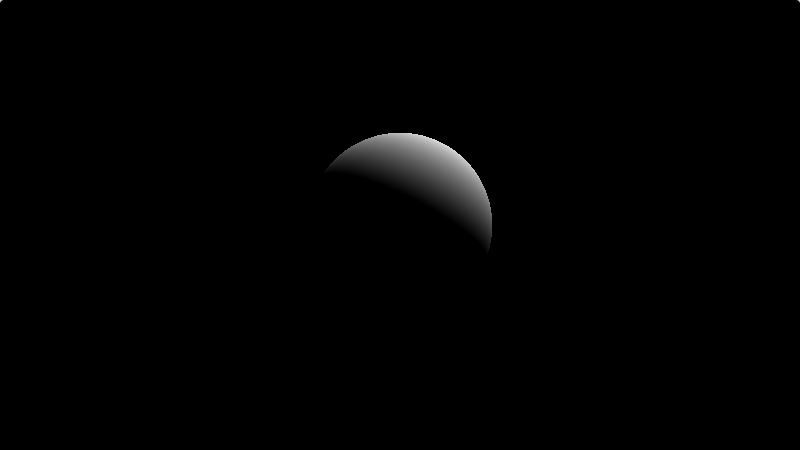
\includegraphics[width=1.0\textwidth]{secciones/imagenes/lightmodel/difusa.png}
  \caption{Intensidad Difusa sobre la esfera.}
  \label{fig:difusse}
\end{figure}
\subsection{Intensidad especular}
Esta intensidad indica como incide la luz reflectada  por la \textit{isosuperficie} en el la dirección del ojo. Definimos \enquote{\(\veebar\)}, como el operador de reflexión\ref{eq:reflexion}. La ecuación final de la \enquote{\textit{Intensidad Especular}} para todas las luces de la escena es,
\[I_e = \sum_{\Vec{l_i}\in L} \Vec{ojo}\cdot_{[0, 1]}\left(\left(\Vec{l_i}-\Vec{p}\right) \veebar \Vec{n}\right)\]
Algunos autores aportan una leve modificación de esta ecuación, aplicando un \textit{homeomorfismo} polinómico con grado exponencial, que es utilizado como factor de brillo\footnote{En \textit{OpenGL}, el brillo por reflexión depende de un parámetro de  \textit{glMaterial}, \textit{GL\_SHININESS}.}, \cite{glmaterial}.
\[h_k:[0,1]\longrightarrow[0,1] , h_k(x)=x^{2^k}\]
\[I_d = \sum_{\Vec{l_i}\in L} h_k\left(\Vec{ojo}\cdot_{[0, 1]}\left(\left(\Vec{l_i}-\Vec{p}\right) \veebar \Vec{n}\right)\right)\]
Donde \(k\in\mathbb{R}^{+}\) y este tiene efecto sobre el radio de rayos reflejados.
\begin{figure}[H]
  \centering
  \captionsetup{justification=centering}%,margin=2cm
  \subfloat[Intensidad especular con \(h_0(x)=x\)]{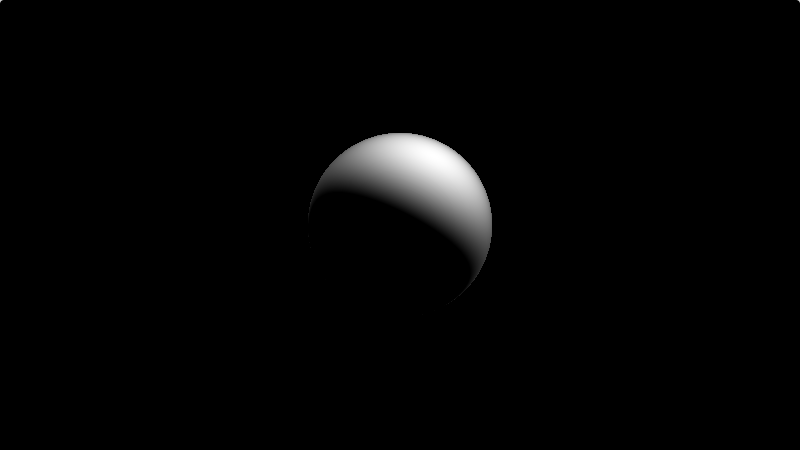
\includegraphics[width=0.30\textwidth]{secciones/imagenes/lightmodel/especular-0.png}}
  \hfill
  \subfloat[Intensidad especular con \(h_1(x)=x^2\)]{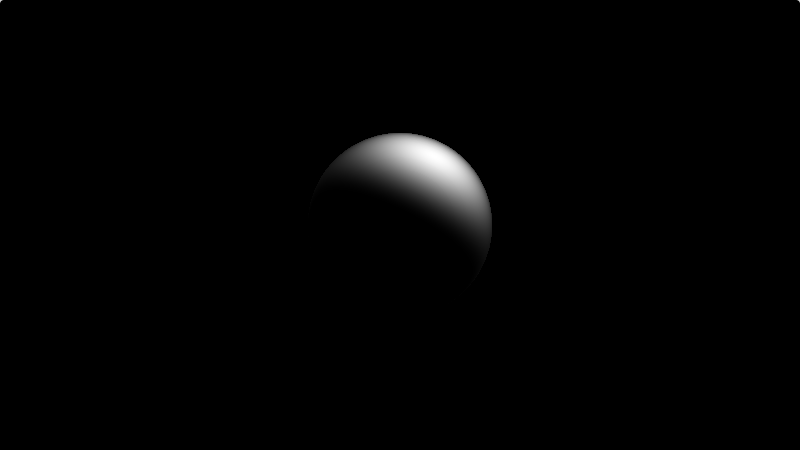
\includegraphics[width=0.30\textwidth]{secciones/imagenes/lightmodel/especular-1.png}}
  \hfill
  \subfloat[Intensidad especular con \(h_3(x)=x^8\)]{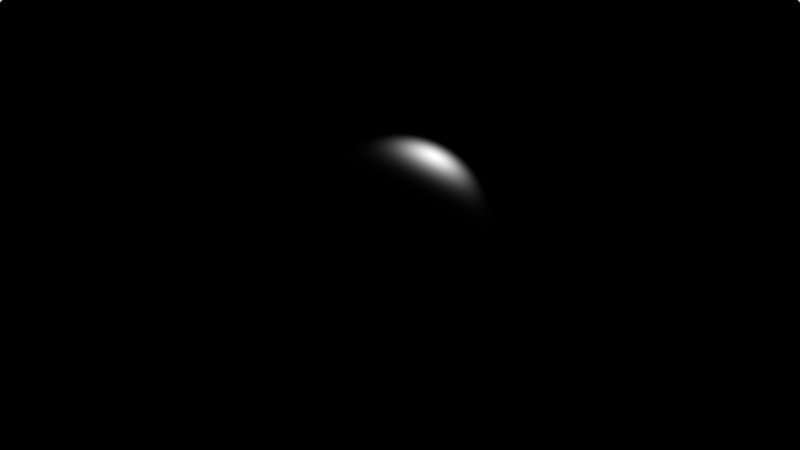
\includegraphics[width=0.30\textwidth]{secciones/imagenes/lightmodel/especular-2.png}}
  \caption{Intensidad Difusa con distintos homeomorfismos}
  \label{fig:specular}
\end{figure}
\subsection{Modelo de Phong}
Resultado final del modelo, definido por la \textit{Intesidad del modelo de Phong}, se calcula como la suma de las intensidades expuestas anteriormente.
\[I_{Phong}=I_a+\sum_{\Vec{l_i}\in L} \mathrlap{\underbrace{\phantom{\Vec{n}\cdot_{[0, 1]}(\Vec{l_i}-\Vec{p})}}_{\text{Intensidad Difusa}}}\Vec{n}\cdot_{[0, 1]}(\Vec{l_i}-\Vec{p}) + \mathrlap{\underbrace{\phantom{h_k\left(\Vec{ojo}\cdot_{[0, 1]}\left(\left(\Vec{l_i}-\Vec{p}\right) \veebar \Vec{n}\right)\right)}}_{\text{Intensidad Especular}}}h_k\left(\Vec{ojo}\cdot_{[0, 1]}\left(\left(\Vec{l_i}-\Vec{p}\right) \veebar \Vec{n}\right)\right)\]
En luces direccionales, el punto se considera estar en el infinito, sustituyéndose \(\Vec{l_i}-\Vec{p}\) por el vector director de la luz direccional \(\Vec{d_i}\). En algunas implementaciones, se utiliza para cada luz, un factor de atenuación que depende de la distancia de la superficie a la luz, esta función converge a cero en el infinito. En caso de utilizar luces direccionales, el valor que tomará  será cero si \(f(d)\) no es constante, anulándose el aporte de \textit{Intensidad Especular} de esta luz.\\\\
En particular, OpenGL\cite{gllight} hace uso de la siguiente función de atenuación:
\[f(d)=\dfrac{1}{k_qd^2+k_ld+k_c}\]
Donde \(k_q,k_l,k_c \in \mathbb{R}^{+}_{0}\) son tres parámetros de atenuación \footnote{Cada parámetro corresponde en OpenGL con un parámetro de la clase \textit{glLight}: \(k_q\) con \textit{GL\_QUADRATIC\_ATTENUATION}; el factor \(k_l\) con \textit{GL\_LINEAR\_ATTENUATION}; finalmente, \(k_c\) con el parámetro, \textit{GL\_CONSTANT\_ATTENUATION}.}.\\\\
La intensidad es un factor, que multiplica al valor del píxel a mostrar, que es tomado del material de la figura\ref{ch:material}, aunque en estos ejemplos, devolveremos como color, el valor de la intensidad, resultando de una imagen en escala de grises.\\\\
Veamos un ejemplo práctico, vamos a añadir dos luces, una direccional desde uno de los laterales de la escena y otra luz, radial. Además vamos a utilizar el \textit{homeomorfismo} \(h_3(x)=x^{2^3}\).\\

\begin{lstlisting}
// Homomorfismo
float h3(float h){return pow(h,pow(2.,3.));}
// Producto escalar normalizado positivo.
float dot01(vec3 a, vec3 b){ 
    return max(dot(a,b)/(normalize(a)*normalize(b)), 0.0);
}
// Modelo de iluminación Phong
float ModeloIluminacion(
    in vec3 direccion,
    in vec3 p
){
    // Calculamos la normal del punto.
    vec3 normal = Normal(p);
    // Emujamos de la superficie
    p = p + normal * 0.1;
    float intensidad = 0.0;
    // Intensidad Ambiente Global
    intensidad += 0.2;
    // Intensidad de cada Luz
    // Luz 1.
    vec3 posicion_luz_1 = vec3(3.0, 3.0, 1.);
    vec3 d_luz_1 = posicion_luz_1 - p;
    vec3 dir_luz_1 = normalize(d_luz_1);
    float dst_luz_1 = length(d_luz_1);
    // Intensidad Difusa
    intensidad += dot01(d_luz_1, normal);
    // Intensidad Especular (Si no es direccional)
    vec3 r_luz_1 = reflect(d_luz_1, normal);
    intensidad += f_difusa(dst_luz_1) * h3(dot01(r_luz_1, direccion));
    
    // Luz 2. Direccional
    vec3 dir_luz_2 = -normalize(vec3(1., 0., 0.));
    // Intensidad Difusa
    intensidad += dot01(dir_luz_2, normal);
    // La intensidad debe ser <= 1.
    return min(intensidad, 1.0);
}
\end{lstlisting}

El enlace del ejemplo: \url{https://www.shadertoy.com/view/wtlBWr}\\
\begin{figure}[H]
  \centering
  \captionsetup{justification=centering}%,margin=2cm
  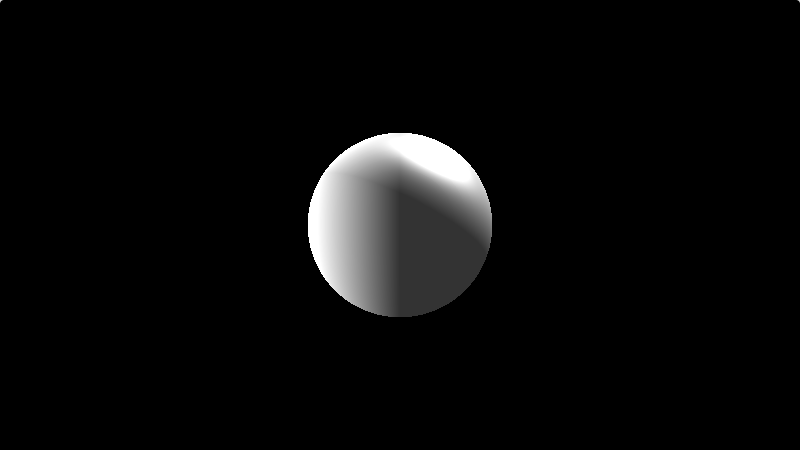
\includegraphics[width=1.0\textwidth]{secciones/imagenes/lightmodel/phong.png}
  \caption{Modelo de Phong sobre la esfera con \(h_3(x)=x^8\).}
  \label{fig:phong}
\end{figure}

\section{Sombras}
Vamos a ver la técnica más sencilla para calcular las sombras, es importante mencionar que hablaremos únicamente de la \textit{umbra} de una la sombra, es decir, cuando la fuente de luz es ocluida completamente por una superficie,  haciendo que esa luz no aporte intensidad.\\\\
Dado un punto punto \(p\) sobre la superficie, lanzaremos otro rayo hacia la luz para ver si este es ocluido, en caso de trazar otro punto \(\Vec{q}\) en esa dirección, la intensidad se mantendrá constante.\\\\
Al lanzar el rayo desde la una isosuperficie, las primeras iteraciones resultan de bolas pequeñas, afectando a la eficiencia del algoritmo, para solucionarlo, separaremos el punto \(\Vec{p}\) de la superficie haciendo uso de la normal de la superficie y un factor de empuje \(k\in\mathbb{R}^{+}_{0}\). Elegido de manera empírica según la escena, se aconseja \(k\in(0,1]\).
\[\Vec{p'}=\Vec{p} + \Vec{n} \cdot k\]
% Imagen Desplazamiento 
Ahora el \textit{Marcher} aceptará un tercer argumento, la distancia máxima recorrida, que anteriormente estaba fijado por la definición \textit{MAXIMO}, de la condición de parada. El tercer argumento: en luces radiales será la distancia del punto a la luz; en luces direccionales, utilizaremos \textit{MAXIMO}.
\newpage
\begin{lstlisting}
// Añadimos un tercer agumento.
float SphereMarching(
    in vec3 ojo, 
    in vec3 direccion,
    float distancia_maxima
){
    float distancia = 0.0;
    for(int i = 0; i < PASOS; ++i){
        vec3 rayo = ojo + direccion * distancia;
        float radio = escena_sdf(rayo);
        if(radio < EPSILON){
            return distancia;
        }
        distancia += radio;
        // Ahora depende del tercer argumento
        if(distancia>distancia_maxima)break;
    }
    return distancia_maxima;
}
\end{lstlisting}

Utilizaremos el modelo de iluminación descrito antes, con una luz radial y otra direccional. Además, utilizaremos un plano en donde proyectar la sombra. La luz direccional es perpendicular al plano.\\
\begin{lstlisting}
// Escena plano + esfera
float escena_sdf(vec3 rayo){
    vec3 pt = rayo - vec3(0., -0.3, 0.);
    vec3 n = normalize(vec3(0., 1., 0.));
    return min(dot(pt, n), length(rayo)-.2);
}

// Modelo Phong + Sombras
float ModeloIluminacion(vec3 direccion, vec3 p){
    // Empujamos de la superficie el punto 
    p = p + Normal(p) * 0.1;
    float intensidad = 0.0;
    // Intensidad Ambiente Global
    intensidad += 0.2;
    // Luz 1. Radial
    vec3 posicion_luz_1 = vec3(3.0, 3.0, 1.);
    vec3 d_luz_1 = posicion_luz_1 - p;
    vec3 dir_luz_1 = normalize(d_luz_1);
    float dst_luz_1 = length(d_luz_1);
    if(SphereMarching(p, dir_luz_1, dst_luz_1) >= dst_luz_1){
        // Intensidad Difusa
        intensidad += dot01(d_luz_1, normal);
        // Intensidad Especular
        vec3 r_luz_1 = reflect(d_luz_1, normal);
        intensidad += f_difusa(dst_luz_1) * h3(dot01(r_luz_1, direccion));
    }
    // Luz 2. Direccional
    vec3 dir_luz_2 =-normalize(vec3(1.,0.,0.));
    if(SphereMarching(p, dir_luz_2, MAXIMO) >= MAXIMO){
        // Intensidad Difusa
        intensidad +=dot01(dir_luz_2,normal);
    }
    return clamp(intensidad, 0.0, 1.0);
}
\end{lstlisting}

Enlace del ejemplo: \url{https://www.shadertoy.com/view/wtfBW8}

\begin{figure}[H]
  \centering
  \captionsetup{justification=centering}%,margin=2cm
  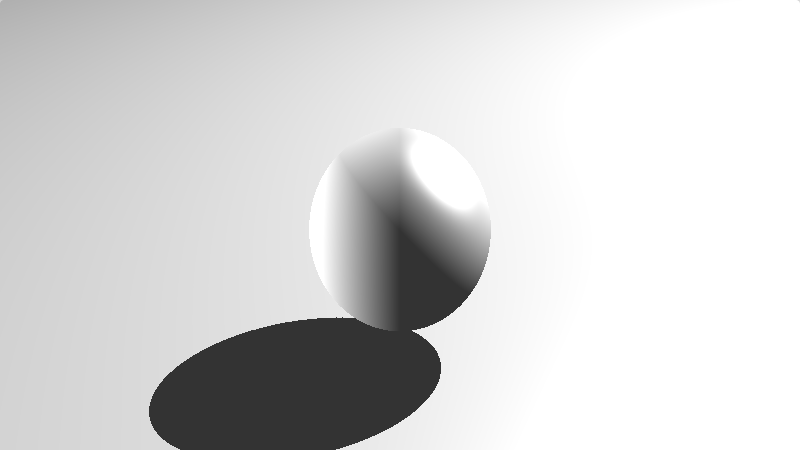
\includegraphics[width=1.0\textwidth]{secciones/imagenes/lightmodel/sombra_dura.png}
  \caption{Modelo de iluminación y sombras sobre la escena definida.}
  \label{fig:shadow}
\end{figure}

Hemos visto como generar la umbra de una sombra, pero no la penumbra, la zona donde llega poca luz pero no está completamente a oscuras. Íñigo Quilez recopila varias de estas aproximaciones \cite{softshadows}.


\newpage
